\thechapter{Experimental results} 


%add images showing light changes w/position

Positioning of the light for optimally rending the lighting is highly dependant on the model, and the area of the model that is being viewed. The effect produced by lighting, and rim lighting in particular, could be further improved by geometry dependent lighting methods described in \cite{lee06}, where the objects are divided into curved surface patches and lighting is applied to each independently. This would enable customization of the lighting to enhance particular aspects of the model and increase the overall quality of the image generated.

\begin{figure}[h]
    \centering
        \begin{subfigure}[b]{0.4\textwidth}
        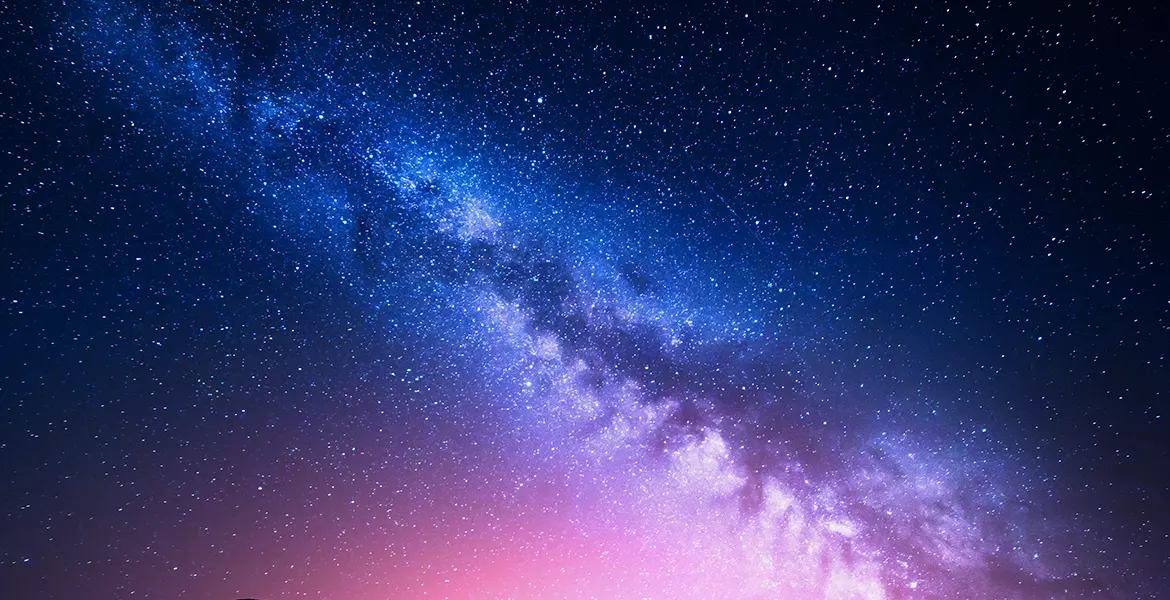
\includegraphics[width=\textwidth]{img/textures/space.png}
        \caption{Initial Texture}
        \label{fig:OriginalSkull}
    \end{subfigure}
    ~
    \centering
    \begin{subfigure}[b]{0.2\textwidth}
        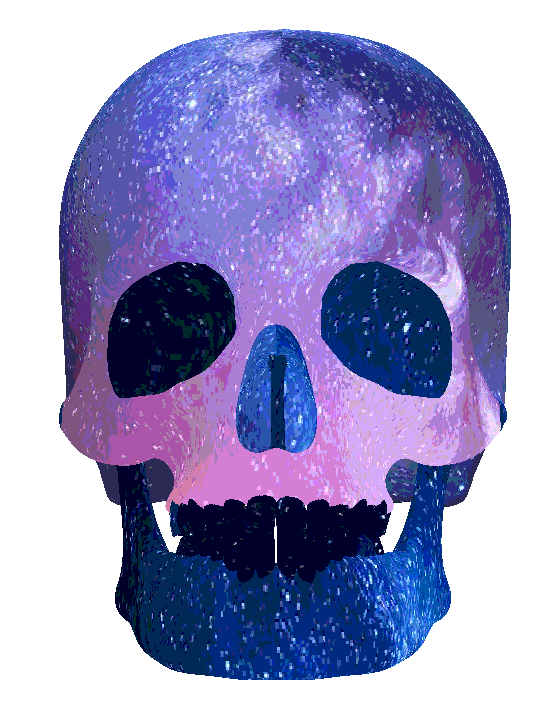
\includegraphics[width=\textwidth]{img/textures/TextureReplacementSkull.png}
        \caption{Skull}
        \label{fig:TextureReplacementSkull}
    \end{subfigure}
     ~
    \centering
    \begin{subfigure}[b]{0.2\textwidth}
        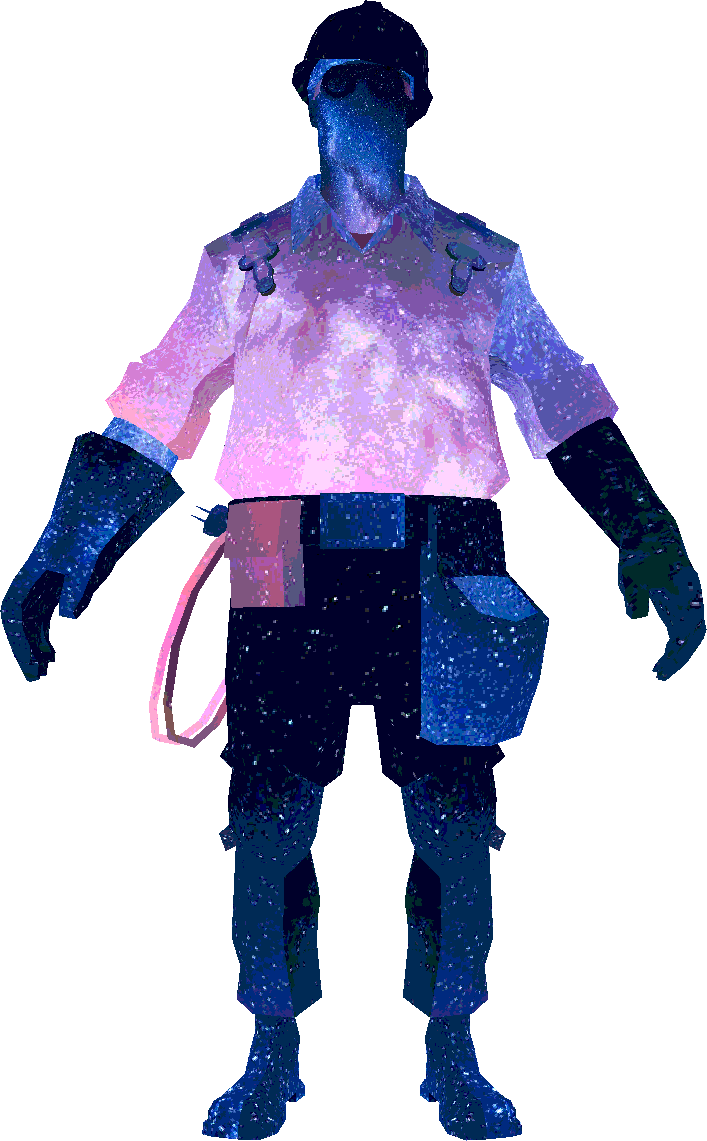
\includegraphics[width=\textwidth]{img/textures/TextureReplacement.png}
        \caption{Engineer}
        \label{fig:TextureReplacement}
    \end{subfigure}
    \caption{Replaced Textures}
    \label{fig:TexturesEngineer}
\end{figure}

Using a photo-realistic image transformed through cel shading as the new texture can produce interesting renders with the same process used for the original textures. While this was not an initial goal for our project it did not require any significant changes to our implementation.